% arara: xelatex
\documentclass[11pt]{article} % размер шрифта
\usepackage{libertine}

\usepackage{tikz} % картинки в tikz
\usepackage{microtype} % свешивание пунктуации

\usepackage{array} % для столбцов фиксированной ширины

\usepackage{indentfirst} % отступ в первом параграфе

\usepackage{multicol} % текст в несколько колонок
\usepackage{verbatim}

\graphicspath{{images/}} % путь к картинкам

\usepackage{sectsty} % для центрирования названий частей
\allsectionsfont{\centering} % приказываем центрировать все sections

\usepackage{amsmath, amssymb} % куча стандартных математических плюшек

\usepackage[top=1cm, left=1cm, right=1cm, bottom=1cm]{geometry} % размер текста на странице

\usepackage{lastpage} % чтобы узнать номер последней страницы

\usepackage{enumitem} % дополнительные плюшки для списков
%  например \begin{enumerate}[resume] позволяет продолжить нумерацию в новом списке
\usepackage{caption} % подписи к картинкам без плавающего окружения figure

\usepackage{circuitikz} % для рисовки электрических цепей

% \usepackage{physics} % do not use it!

\usepackage{fancyhdr} % весёлые колонтитулы
\pagestyle{empty}
%\lhead{ФМТ}
%\chead{}
%\rhead{КЛШ-2019}
%\lfoot{}
%\cfoot{}
%\rfoot{\thepage/\pageref{LastPage}}
%\renewcommand{\headrulewidth}{0.4pt}
%\renewcommand{\footrulewidth}{0.4pt}



\usepackage{todonotes} % для вставки в документ заметок о том, что осталось сделать
% \todo{Здесь надо коэффициенты исправить}
% \missingfigure{Здесь будет картина Последний день Помпеи}
% команда \listoftodos — печатает все поставленные \todo'шки

\usepackage{booktabs} % красивые таблицы
% заповеди из документации:
% 1. Не используйте вертикальные линии
% 2. Не используйте двойные линии
% 3. Единицы измерения помещайте в шапку таблицы
% 4. Не сокращайте .1 вместо 0.1
% 5. Повторяющееся значение повторяйте, а не говорите "то же"

\usepackage{fontspec} % поддержка разных шрифтов
\usepackage{polyglossia} % поддержка разных языков

\setmainlanguage{russian}
\setotherlanguages{english}

\setmainfont{UbuntuMono Nerd Font}
\usepackage{unicode-math}
\setmathfont{Fira Math}

% \setmainfont{Linux Libertine O} % выбираем шрифт
% можно также попробовать Helvetica, Arial, Cambria и т.Д.
% перешли на \usepackage{libertine}

% чтобы использовать шрифт Linux Libertine на личном компе,
% его надо предварительно скачать по ссылке
% http://www.linuxlibertine.org/

% \newfontfamily{\cyrillicfonttt}{Linux Libertine O}
% пояснение зачем нужно шаманство с \newfontfamily
% http://tex.stackexchange.com/questions/91507/

\AddEnumerateCounter{\asbuk}{\russian@alph}{щ} % для списков с русскими буквами
\setlist[enumerate, 2]{label=\asbuk*),ref=\asbuk*} % списки уровня 2 будут буквами а) б) ...


% делаем короче интервал в списках
\setlength{\itemsep}{0pt}
\setlength{\parskip}{0pt}
\setlength{\parsep}{0pt}


\newcommand{\shortname}{ФМТ: тур 3}

\begin{document}


\section*{Правила игры уголки}
\begin{enumerate}
    \item Один игрок/игрица играет кружочками, второй — треугольниками. 
    \item Право первого хода определяется на "камень-ножницы-бумага" (КНБ). В первой партии ходит выигравший в КНБ, во второй - проигравший.
    \item Поле стандартное — 8 на 8 в клетку. 
    \item За один ход игрок/игрица выставляет одну свою фигуру на поле. 
    \item Размещать свои фигуры можно только в свободные клетки.
    \item Если 4 одинаковые фигуры расположены в углах прямоугольника, то на следующем ходу игрок/игрица может занять его.
    \item Прямоугольник может быть повернутым на \textbf{произвольный угол} относительно границ игрового поля!!!
    \item Ход захвата прямоугольника: \begin{enumerate}
        \item Закрашиваются фигуры в углу прямоугольника
        \item На месте пустых клеток \textbf{внутри прямоугольника}\footnote{Клетка находится внутри прямоугольника, если ее центр лежит внутри ограничеваемого прямоугольника} ставятся фигуры, которые принадлежат игроку
        \item Можно захватить прямоугольник, даже если внутри его есть чужые фигуры или нет пустых клеток.
    \end{enumerate}
    \item Когда все поле \textbf{замостится фигурами}, у каждого игрока есть право захватить еще по одному прямоугольнику.
    \item Финальное число очков - это число закрашенных фигур игрока.
\end{enumerate}

\begin{figure}[h!]
\begin{minipage}{0.5\textwidth}
    \centering{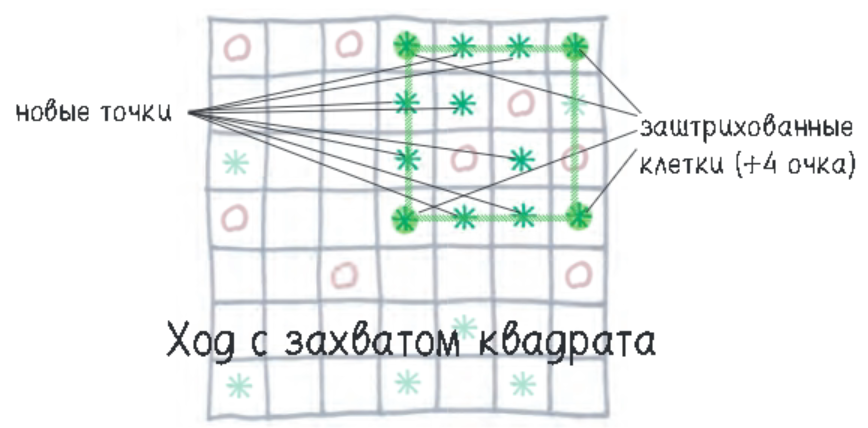
\includegraphics[scale=0.5]{1.png}}
    \caption{Ход захвата прямоугольника}
\end{minipage}
\begin{minipage}{0.5\textwidth}
    \centering{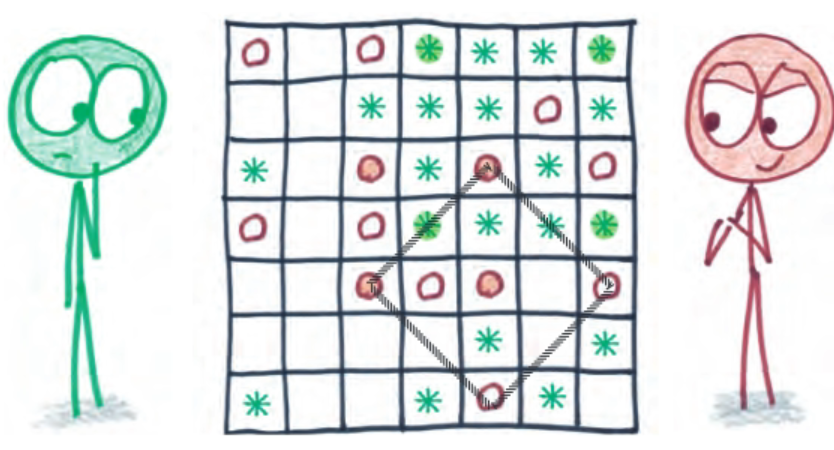
\includegraphics[scale=0.5]{2.png}}
    \caption{Ход захвата прямоугольника с поворотом}
\end{minipage}
\end{figure}

Счет в игре - это разница очков. Если по итогам партии у игрока/игрицы
\begin{enumerate}
    \item Больше очков, чем у противника  -- победа
    \item Столько же очков -- ничья
    \item Меньше очков -- поражение
\end{enumerate}

\newpage
\section*{Организация тура}

Игровой тур состоит из четырёх фаз: объяснение правил, сыгрывание, индивидуальные партии, командные партии.

\begin{enumerate}
    \item Во время сыгрывания команда и вольные стрелки объединяются и играют тренировочные партии между собой. 
    Судьи отвечают на вопросы игроков. На объяснение правил и сыгрывание команд отводится примерно 20 минут. 
    \item После сыгрывания капитан каждой команды объявляет основной состав команды из четырёх человек и вольных стрелков в любом количестве.
    \item Во время индивидуальных партий основной состав команд А и Б делятся на пары: АБ, АБ, АБ, АБ. 
    \item Вольные стрелки играют как единый дополнительный пятый игрок своей команды. 
    Вольные стрелки играют против вольных стрелков. 
    \item За индивидуальный этап каждая из 5 пар (4 пары основных участиников + вольные стрелки) играют две партии.
    \item В каждой партии индивидуального тура разыгрывается 1 очко. Если есть победитель, то он/она получает это очко. В случае ничьи оба игрока/игрицы делят 1 очко между поровну между собой.
    \item За индивидуальный этап команда получает сумму очков, набранных всеми её игроками. 
    \item На индивидуальный этап отводится примерно 15 минут\footnote{Если время индивидуального этапа позволяет и оба игрока в паре и судьи согласны, то игроки могут сыграть ещё пару партий, но уже не в счет встречи}.
    \item На командном этапе команда вместе с вольными стрелками играет как единое целое. 
    \item Ход выполняет капитан команды у доски. На обсуждение каждого хода отводится 40 секунд. 
    \item В каждой партии командного тура разыгрывается 6 очков. Если есть команда-победитель, то он/она получает шесть очков. В случае ничьи обе команды получают по 3 очка.
    \item Итоговые очки за игровой тур равны сумме очков за индивидуальный и командный этапы.
    \item Судьи отмечают в протоколе имена игроков основного состава в индивидуальном этапе, очки, которые они заработали, 
    а также очки, набранные вольными стрелками, и очки в командном этапе. Не забывайте отметить капитанов!
\end{enumerate}

\newpage
\newcommand\sqw{1}
\newcommand\square[4][1]{\fill[#4] (#2*\sqw,#3*\sqw) rectangle +(#1*\sqw,#1*\sqw);}
\renewcommand\sqw{1.5}
\begin{center}
\begin{tikzpicture}
    \draw[step=\sqw] (0,0) grid (8*\sqw, 8*\sqw);
\end{tikzpicture}
\vfill
\begin{tikzpicture}
    \draw[step=\sqw] (0,0) grid (8*\sqw, 8*\sqw);
\end{tikzpicture}
\end{center}


\end{document}